% arara: pdflatex
% arara: convert: {density: 160, otheroptions: -dispose previous -delay 40 -loop 1, format: gif}
% arara: showfile: {format: gif}
% !Mode:: "TeX:UTF-8:Main"
\documentclass{article}
\usepackage[utf8]{inputenc} %probably not needed ...
\usepackage[T1]{fontenc}
\usepackage{geometry}
\geometry{papersize={128mm,96mm},margin=0.5cm} %\textwidth=11.8, \textheight=8.6
\usepackage[x11names,svgnames]{xcolor}
\usepackage{tikzducks}

\newcommand{\welshduck}[2]{%
	\begin{scope}[scale=.5,xshift=#1em,yshift=#2ex]
		\clip (0,0) -- ++(2.2,0) -- ++(0,2.6) -- ++(-2.2,0) -- cycle;
		\duck[crazyhair=red]	
	\end{scope}%
}

\begin{document}
\centering

\begin{tikzpicture}
\foreach \x in {0,10,...,60}{
	\foreach \y in {0}{		
		\welshduck{\x}{\y}
	}
}
\end{tikzpicture}
\newpage
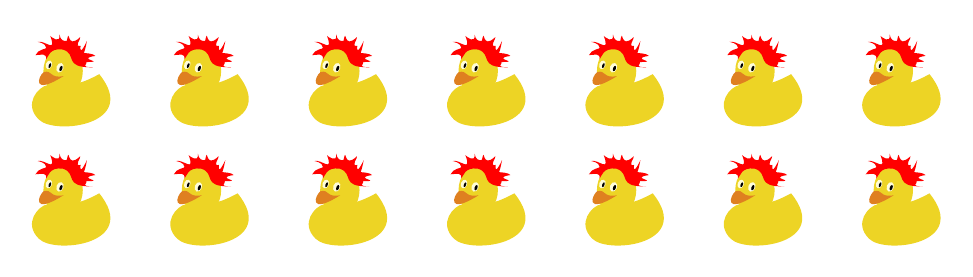
\begin{tikzpicture}
\foreach \x in {0,10,...,60}{
\foreach \y in {0,20}{		
	\welshduck{\x}{\y}
}
};
\end{tikzpicture}
\newpage
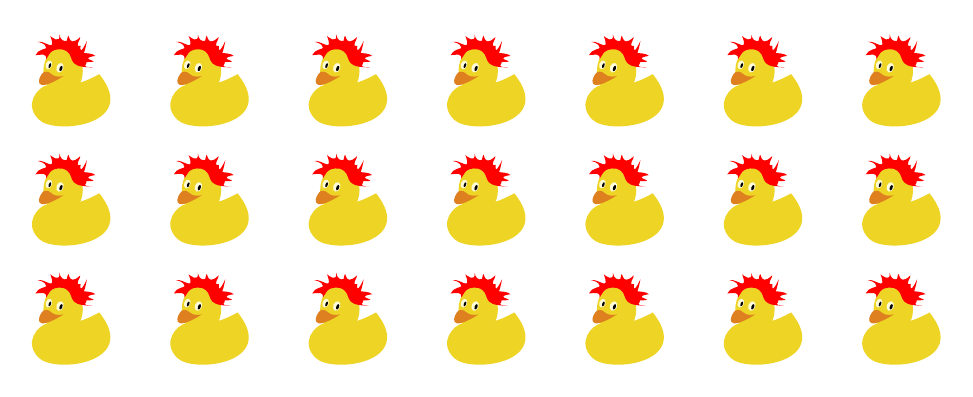
\begin{tikzpicture}
\foreach \x in {0,10,...,60}{
\foreach \y in {0,20,40}{		
	\welshduck{\x}{\y}
}
};
\end{tikzpicture}
\newpage
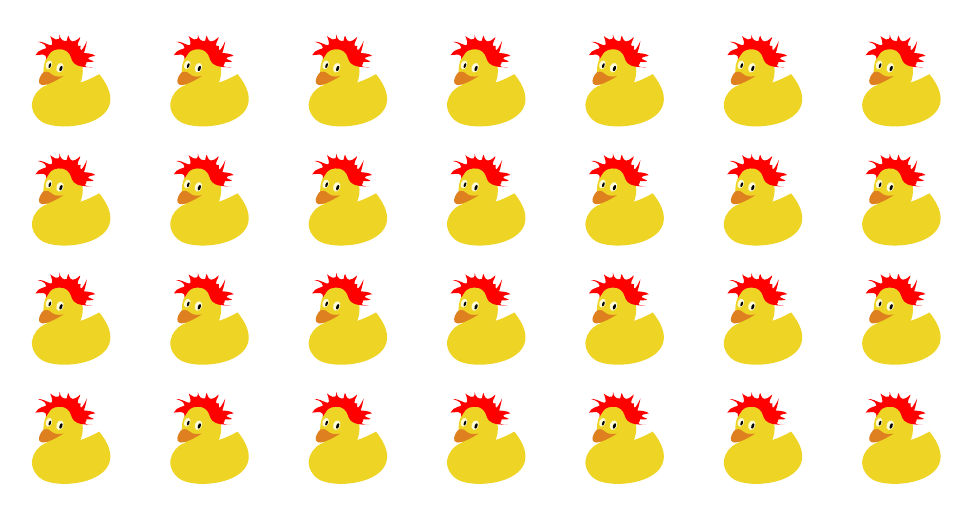
\begin{tikzpicture}
	\foreach \x in {0,10,...,60}{
		\foreach \y in {0,20,...,60}{		
			\welshduck{\x}{\y}
		}
	}
\end{tikzpicture}
\newpage
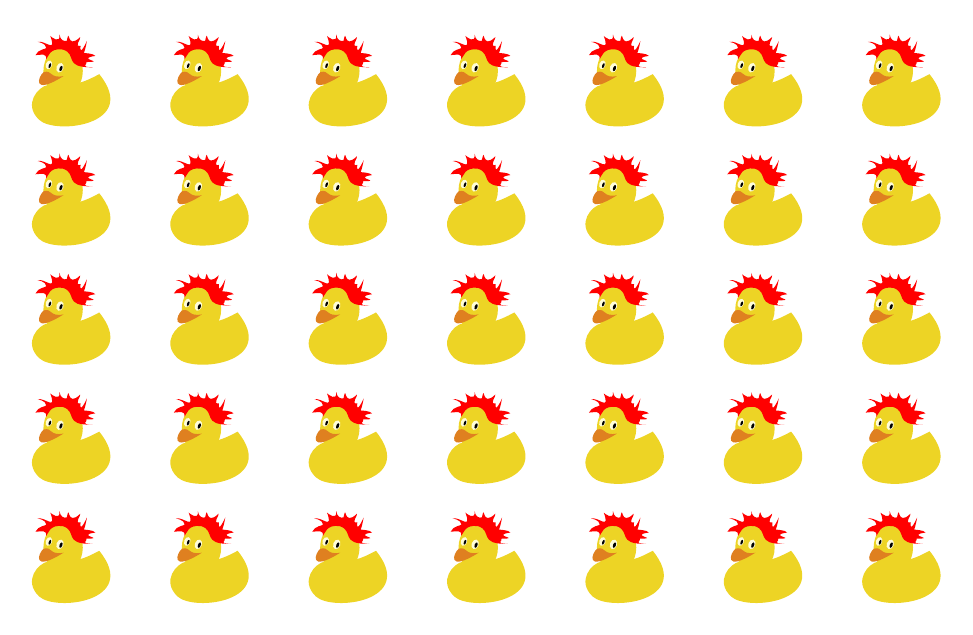
\begin{tikzpicture}
\foreach \x in {0,10,...,60}{
	\foreach \y in {0,20,...,80}{		
		\welshduck{\x}{\y}
	}
}
\end{tikzpicture}
\newpage
\begin{tikzpicture}
	\foreach \x in {0,10,...,60}{
		\foreach \y in {0,20,...,100}{		
			\welshduck{\x}{\y}
		}
	};
	\node[draw, inner sep=2\pgflinewidth] at (16.6em, 29ex) {
\includegraphics[width=.75\textwidth]{Flag_of_Wales}};
\end{tikzpicture}
\end{document}